\documentclass[11pt]{article}
\usepackage[a4paper,margin=2.3cm]{geometry}
%\usepackage[T1]{fontenc}
\usepackage[utf8]{inputenc}
%\usepackage{lmodern}
\usepackage{amsmath,amssymb,amsthm}
\usepackage{graphicx}
\usepackage{booktabs}
\usepackage{multirow}
\usepackage[numbers,sort&compress]{natbib}
\usepackage{microtype}
\usepackage{xcolor}
\usepackage[colorlinks=true,linkcolor=blue!50!black,citecolor=blue!50!black,urlcolor=blue!50!black]{hyperref}

\newtheorem{proposition}{Proposition}
\newtheorem{theorem}{Theorem}
\newtheorem{corollary}{Corollary}
\theoremstyle{remark}
\newtheorem{remark}{Remark}
\theoremstyle{definition}
\newtheorem{assumption}{Assumption}

\newcommand{\Prb}{\mathbb{P}}
\newcommand{\E}{\mathbb{E}}

\title{Certified Adaptive Examination of Peripheral Blood Smears:\\
When Information-Gain Stopping Fails, and What Can Be Guaranteed Instead}
\author{%
\begin{tabular}{c}
\textbf{Author:} Qudrat Ullah\\
\textbf{Supervisor:} Dr.\ Bal\'azs Harangi\\[4pt]
\normalsize Faculty of Informatics, University of Debrecen, Hungary\\
\normalsize \href{mailto:qudratafridi@mailbox.unideb.hu}{qudratafridi@mailbox.unideb.hu}
\end{tabular}}
\date{Preprint, \today}

\begin{document}
\maketitle

\begin{abstract}
Automated examination of peripheral blood smears increasingly selects which fields to inspect and when to stop. We ask what such a procedure can guarantee about the part of the specimen it did \emph{not} examine. Hypotheses, decision rules and analysis code were frozen in five git tags before the corresponding data were generated. The evidence comprises about 67,500 confirmatory simulated specimens, most built from 28,280 expert-labelled cells, an external dataset, and real, fully annotated bone-marrow regions.
\textbf{(i)} A reimplementation of information-saturation stopping (InfoDPP-PAC) halts at about 16\% of the specimen, whatever the number of decision-changing fields. Its halting signal loses its association with blasts as cells are pooled into fields (AUC 0.78 at one cell per field, 0.52 at twenty). A teacher trained on the same pooled representation remains informative (0.98 to 0.83). With one critical field among 200 and ten cells per field, InfoDPP-PAC misses 76\% of positive specimens, against 85\% for uniform sampling of the same size.
\textbf{(ii)} When pre-inspection features carry no information about where rare evidence lies, every strategy has worst-case miss probability at least $\binom{N-k}{n}/\binom{N}{n}$. Certifying the absence of a single critical field at $\alpha=0.05$ therefore requires examining 95\% of the fields.
\textbf{(iii)} Certifying that the blast proportion exceeds a threshold (0.10, ICC 2022; 0.20, WHO 2022) is feasible with ALPHA and importance-weighted betting tests. False certification stayed at or below 0.04 for every valid design and population size from 500 to 4,000 cells. The cost is set by the margin to the threshold, not by the population size. At a margin of 0.05, uniform sampling needed 165--420 cells and classifier-driven sampling 35--58\% as many; within 0.02 of the threshold, uniform sampling of 2,000- to 4,000-cell specimens needed 1,000--2,000 cells. An uncorrected adaptive design certified falsely in 89--99\% of boundary specimens, and a 100-cell count called ``above'' in 41--45\% of specimens lying on the threshold.
\textbf{(iv)} Validity survived an acquisition shift that cut classifier blast recall from 0.91 to 0.34, but efficiency did not (195 vs.\ 110 cells). The unit of analysis decides validity. Treating the cells of sampled fields as individual draws inflates false certification, modestly at the clustering measured in real marrow and severely under strong clustering. Averaging field proportions when fields differ in size certified falsely in 32--38\% of boundary specimens, even with no association between size and proportion. Weighting fields by known cell counts, or a bounded assorter when counts are unknown, restores validity. Guarantees about unexamined material therefore come from the sampling design and the unit of analysis, not from model confidence. We state what the experiments do not establish, including clinical validity.
\end{abstract}

\section{Introduction}
A peripheral blood smear contains far more cells than any examiner inspects. A manual differential usually counts 100 or 200 leukocytes, and the statistical variability that this implies has been known for decades \cite{rumke1978}. Automated systems add a new degree of freedom: they choose which fields to look at and decide when enough has been seen. For diagnostic questions that hinge on rare cells, such as the proportion of blasts relative to a classification threshold \cite{khoury2022who,arber2022icc}, the relevant question is not how accurate the classifier is on the fields it examined, but what can be said about the fields it did not examine.

Adaptive stopping rules based on \emph{information saturation} address this question implicitly. They stop when additional fields are expected to add little information about the specimen as the selector's embedding represents it. InfoDPP-PAC \cite{mittal2026infodpp} is a recent, carefully constructed instance for whole-slide histopathology. It combines Gaussian-process relevance, determinantal diversity and a PAC-style halting certificate, and its authors state clearly that the certificate bounds residual information in the selection objective, not downstream diagnostic performance. That distinction is the starting point of this paper. Saturation of information about the embedding does not imply that the decision-relevant evidence has been seen, especially when that evidence is rare.

We study this gap in the setting of peripheral blood smears and blast counting, and ask four research questions:
\begin{itemize}
\item[\textbf{RQ1}] Does information-saturation stopping fail systematically when decision-changing evidence is rare?
\item[\textbf{RQ2}] Why does certifying the \emph{absence} of rare evidence require near-exhaustive examination in the worst case?
\item[\textbf{RQ3}] How many cells must be examined to certify a threshold decision under adaptive sampling?
\item[\textbf{RQ4}] Where do the assumptions of anytime-valid audit methods break on real blood-smear data?
\end{itemize}

\paragraph{Contributions.}
\begin{enumerate}
\item A pre-registered evaluation of information-saturation stopping on specimens assembled from real expert-labelled cells with controlled rarity and dilution. It shows that the stopping point does not depend on how much critical evidence is present, and that its halting signal decouples from critical evidence as cells are pooled into fields, although a teacher with access to the same pooled representation still detects it (RQ1). One of the Part I predictions failed (three of the 20 pre-registered hypotheses overall), and these failures are reported as such.
\item A worst-case lower bound, a direct application of Yao's minimax principle \cite{yao1977}. It shows that near-exhaustive examination is required of \emph{every} strategy that lacks location information, not only of uniform sampling (RQ2).
\item An evaluation of design-based, anytime-valid certification of blast-proportion assertions using ALPHA \cite{stark2023alpha} and importance-weighted betting under adaptive sampling \cite{shekhar2023rlfa}. We quantify validity and cost for populations of 500 to 4,000 cells, and the failure of uncorrected adaptive designs and conventional counts (RQ3).
\item An empirical examination of the assumptions behind these methods (RQ4): classifier-error heterogeneity, acquisition shift, and spatial clustering of blasts, the last measured in real smear regions in which every cell was annotated, and unequal field sizes. For the latter we give two valid constructions: a weighted test when cell counts are known, and a bounded assorter when only an upper bound is known. We separate the assumptions that matter for validity from those that matter only for efficiency.
\end{enumerate}

\paragraph{Scope.} This is a methodological study. The ``expert'' who verifies sampled cells is simulated with the datasets' expert labels, most specimens are composites of real single-cell images, and no result here establishes clinical diagnostic validity.

\section{Related work}
\paragraph{Variability of cell counts.} The binomial and finite-population variability of manual differentials, and the resulting uncertainty of low-frequency cell types, were characterised by R\"umke \cite{rumke1978}. Our conventional-count baseline makes that variability concrete near a diagnostic threshold. For the absence of rare events, the ``rule of three'' bounds an event rate after zero observed events \cite{hanley1983}; Proposition~\ref{prop:uniform} is its finite-population, design-based counterpart.

\paragraph{Adaptive selection with stopping.} InfoDPP-PAC \cite{mittal2026infodpp}, a recent preprint that has not been peer reviewed and for which no code is released, selects whole-slide image patches greedily under a blended information-gain and relevance objective, and stops when the maximal information gain among unselected patches falls below a concentration-corrected threshold. It was evaluated on gastrointestinal whole-slide images with selection-quality metrics. We reimplement its halting rule as the object of study, not as a straw man. Automated blast recognition itself is well studied \cite{matek2019aml}; our question concerns examination and inference, not classification accuracy.

\paragraph{Risk-limiting audits and betting.} Risk-limiting audits test assertions about finite populations from a sample, with a guaranteed bound on the probability of confirming a false assertion \cite{lindeman2012gentle}. ALPHA \cite{stark2023alpha} turns such assertions into bounded-mean tests using an \emph{assorter}, and constructs a test supermartingale for sampling without replacement. Betting-based confidence sequences \cite{waudbysmith2024betting} provide the underlying anytime-valid machinery, through Ville's inequality \cite{ville1939}. Shekhar et al.\ \cite{shekhar2023rlfa} extend this to weighted, adaptive sampling without replacement: they use importance-weighted observations and allow side information both in the sampling distribution and as control variates. Stratified extensions \cite{spertus2024stratified} are relevant when a specimen is naturally partitioned. Prediction-powered inference \cite{angelopoulos2023ppi} and prediction-powered e-values \cite{csillag2025ppe} combine model predictions with a verified subset, and active statistical inference \cite{zrnic2024active} uses a model to choose which units to label. Prediction-powered and active inference give fixed-sample intervals for a superpopulation parameter, whereas the audit tests used here are anytime-valid statements about one finite specimen. Prediction-powered e-values bring predictions into the e-value framework. We did not implement prediction-powered e-values; side information enters our tests only through the sampling distribution and control variates.

\section{Setting}
A specimen consists of $N$ fields. Field $i$ holds $m_i$ cells, $B_i$ of them blasts, so there are $M=\sum_i m_i$ cells in total. Cell $j$ has a blast indicator $b_j\in\{0,1\}$, and the specimen's blast proportion is $p=M^{-1}\sum_j b_j=\sum_i B_i/\sum_i m_i$. Most experiments use equal field sizes, $m_i=m$; Section~\ref{sec:cert} treats unequal sizes, which real fields have. We distinguish three estimands, which the literature sometimes conflates:
\begin{enumerate}
\item \emph{Detection}: has at least one critical field (a field with at least one blast) been examined?
\item \emph{Estimation}: what is $p$?
\item \emph{Threshold certification}: is $p>\theta$, for a stated threshold $\theta$?
\end{enumerate}
We use $\theta=0.10$, the blast percentage at which the ICC 2022 separates myelodysplastic syndrome with excess blasts from MDS/AML (and, in the presence of AML-defining genetic abnormalities, from AML) \cite{arber2022icc}, and $\theta=0.20$, the WHO 5th-edition blast threshold for acute myeloid leukemia without defining genetic abnormalities \cite{khoury2022who}. Both classifications count certain blast equivalents (for example promonocytes); our labels count blast classes only. They are analysed separately and never pooled. These thresholds are inputs to a statistical procedure; the study does not validate them or any diagnosis.

An examiner selects fields sequentially. Selection may use pre-inspection features $x$ (for instance embeddings) and past verified labels, and may be randomised. A selected field is \emph{verified}: the true labels of all its cells are revealed. All probabilities below are over the examiner's randomisation, conditional on the fixed specimen. The guarantees are therefore finite-population and design-based. They hold for every specimen in the stated class and say nothing about a population of patients.

\section{Why saturation cannot certify absence (RQ2)}\label{sec:theory}
Let $C\subseteq[N]$ be the set of critical fields, with $k=|C|$, and let $M_n$ be the event that none of them is among the (at most) $n$ examined fields. Define
\[
h(N,k,n)=\binom{N-k}{n}\Big/\binom{N}{n}=\prod_{i=0}^{k-1}\frac{N-n-i}{N-i}.
\]

\begin{proposition}[Uniform sampling]\label{prop:uniform}
Under simple random sampling of $n$ fields without replacement, $\Prb(M_n\mid C)=h(N,k,n)$ exactly. For $k=1$ this equals $1-n/N$, so $\Prb(M_n)\le\alpha$ if and only if $n\ge\lceil(1-\alpha)N\rceil$. Moreover, $\big(1-\tfrac{n}{N-k+1}\big)^k\le h\le(1-n/N)^k$, so $n\ge N(1-\alpha^{1/k})$ suffices.
\end{proposition}

\begin{assumption}[No location information]\label{ass:A}
For the given features $x$, every placement $C$ with $|C|=k$ is possible.
\end{assumption}

\begin{theorem}[Minimax lower bound]\label{thm:minimax}
Under Assumption~\ref{ass:A}, every policy (adaptive or not, randomised or not) that examines at most $n$ fields satisfies
\[
\max_{|C|=k}\Prb_\pi(M_n\mid x,C)\ \ge\ h(N,k,n).
\]
Uniform sampling attains this bound for every $C$. Every deterministic policy has worst-case miss probability $1$ whenever $n\le N-k$.
\end{theorem}
\begin{proof}[Proof sketch]
Fix the examiner's randomness $u$. On the run in which every examined field is negative, the policy's inputs are determined by $u$, so it examines a fixed set $A(u)$ with $|A(u)|\le n$. For any $C$, the actual run coincides with this all-negative run up to the first critical field it would reach, so the examiner misses $C$ exactly when $C\cap A(u)=\emptyset$. Averaging over a uniformly random $C$, which Assumption~\ref{ass:A} permits, gives a miss probability of at least $\binom{N-n}{k}/\binom{N}{k}=h(N,k,n)$. Since the maximum over $C$ is at least this average, the bound follows. The full proof is in Appendix~\ref{app:proof}.
\end{proof}

\begin{corollary}[Unknown $k$]\label{cor:unknown}
If an examiner declares ``no critical evidence'' whenever it has examined none, and this declaration must be wrong with probability at most $\alpha$ for every non-empty $C$, then, under Assumption~\ref{ass:A}, it must examine at least $\lceil(1-\alpha)N\rceil$ fields. The reason is that $C\subseteq C'$ implies $M_n(C')\subseteq M_n(C)$ pathwise, so the worst case is $k=1$.
\end{corollary}

\begin{remark}[Imperfect verification]
If verification detects an examined critical field only with probability $1-\beta$, independently of selection, then for $k=1$ under uniform sampling the miss probability is $1-(1-\beta)n/N$, which equals $\beta$ at $n=N$. Absence therefore cannot be certified at level $\alpha<\beta$ even by a census.
\end{remark}

Figure~\ref{fig:partII} shows the resulting requirement. Informative features (the failure of Assumption~\ref{ass:A}) allow a search to beat this bound, but only through a model of where critical evidence appears, and that model is not itself certified. Section~\ref{sec:partI} shows how quickly such information disappears when cells are pooled into fields. Section~\ref{sec:rq4} shows it failing under acquisition shift. The bound is also specific to detecting the \emph{presence} of rare evidence: making ``$p>\theta$'' true requires more than $\theta M$ blasts, which cannot be hidden in a single field. This is why the threshold reformulation of Section~\ref{sec:cert} escapes it.

All statements were checked exactly, using rational arithmetic (for all $N\le120$, and $N\le300$ when $k=1$) and, for $N\le7$, by solving the zero-sum search game as a linear program, whose value equalled $h(N,k,n)$ in every case. The code is in \texttt{scripts/17\_part2\_verify.py}.

\begin{figure}[t]
\centering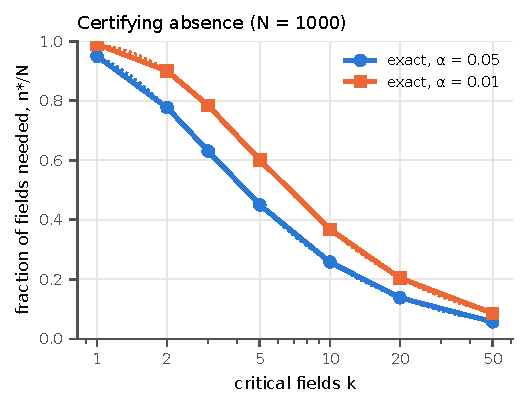
\includegraphics[width=0.48\linewidth]{figures/fig2_partII.pdf}
\caption{Fraction of fields $n^*/N$ that any strategy without location information must examine to certify the absence of $k$ critical fields ($N=1000$; exact hypergeometric values, solid; sufficient closed form $1-\alpha^{1/k}$, dotted). The values depend only weakly on $N$.}\label{fig:partII}
\end{figure}

\section{Certifying a threshold assertion (RQ3)}\label{sec:cert}
Following \cite{stark2023alpha}, define the assorter $a_j=b_j/(2\theta)\in[0,1/(2\theta)]$. Then $\bar a>1/2\iff p>\theta$, so the assertion becomes a one-sided test of $H_0:\bar a\le 1/2$ for a bounded finite population. The observation unit is the field: an expert verifies every cell in a sampled field, the field mean of the assorters is observed, and with equal field sizes the population mean over fields equals $\bar a$. Unequal sizes are treated at the end of this section.

\paragraph{Uniform sampling.} ALPHA constructs a non-negative supermartingale under $H_0$ for sampling without replacement \cite{stark2023alpha}. Rejecting when it exceeds $1/\alpha$ controls the false-certification probability at $\alpha$ for any data-dependent stopping time, by Ville's inequality.

\paragraph{Adaptive sampling.} Write the target as a weighted mean $\sum_i w_i f_i$ over fields, with known weights $w_i>0$, $\sum_i w_i=1$, and field values $f_i\in[0,1]$; with equal field sizes, $w_i=1/N$ and $f_i=B_i/m$, so $\sum_i w_if_i=p$. Let $q_t$ be any predictable distribution over the unsampled fields that is strictly positive on all of them, and let $I_t$ be the field drawn at step $t$. Following Shekhar et al.\ \cite{shekhar2023rlfa}, the importance-weighted observation $Z_t=w_{I_t}f_{I_t}/q_t(I_t)$ has conditional mean equal to the mass not yet sampled, $\sum_{i\ \text{unsampled}}w_if_i$. Under $H_0:p\le\theta$ this is at most $\mu_t=\theta-\sum_{s<t}w_{I_s}f_{I_s}$, the mass the null allows to remain. A betting process $W_t=\prod_{s\le t}(1+\lambda_s(Z_s-\mu_s))$ with predictable, non-negative bets $\lambda_s$, bounded so that wealth cannot become negative, is then a test supermartingale under $H_0$, whatever the classifier does. We use their prop-MS sampler, $q_t(i)\propto w_iS_i$ with a floor, where $S_i$ is the field's mean classifier score; approximate-Kelly bets; and, as a variant, a zero-mean control variate built from $S$. Validity requires only that $q_t$ is known and positive and that labels come from verification. The classifier affects efficiency, not validity.

\paragraph{Fields of unequal size.} The field-mean assorter above averages field \emph{proportions}. When field sizes differ, that average is $N^{-1}\sum_iB_i/m_i$, which is not $p$.

\begin{proposition}[Unequal field sizes]\label{prop:unequal}
Let field $i$ hold $m_i$ cells, $B_i$ of them blasts, and let $p=\sum_iB_i/\sum_im_i$.
\begin{enumerate}
\item[(a)] \emph{Counts known.} If every $m_i$ is known before verification, set $w_i=m_i/M$ and $f_i=B_i/m_i$ (fields with $m_i=0$ are dropped). Then $\sum_iw_if_i=p$, and the weighted betting test above is valid for $H_0:p\le\theta$.
\item[(b)] \emph{Only a bound known.} If only $m_i\le m_{\max}$ is known, define
\[
a_i=\frac{B_i-\theta m_i+\theta m_{\max}}{m_{\max}}.
\]
Then $a_i\in[0,1]$ and $N^{-1}\sum_ia_i>\theta\iff p>\theta$. Equal-weight ALPHA or betting on $a_i$ with null mean $\theta$ is therefore valid.
\end{enumerate}
\end{proposition}
\begin{proof}
(a) $\sum_iw_if_i=\sum_i(m_i/M)(B_i/m_i)=p$, and the construction of Shekhar et al.\ requires only known positive weights and $f_i\in[0,1]$.
(b) Since $0\le B_i\le m_i\le m_{\max}$, we have $a_i\ge\theta(m_{\max}-m_i)/m_{\max}\ge0$ and $a_i\le\{(1-\theta)m_i+\theta m_{\max}\}/m_{\max}\le1$. Summing, $\sum_ia_i=(\sum_iB_i-\theta M)/m_{\max}+N\theta$, so $N^{-1}\sum_ia_i>\theta$ if and only if $\sum_iB_i>\theta M$.
\end{proof}

In (b), the margin $N^{-1}\sum_ia_i-\theta=(p-\theta)\bar m/m_{\max}$ shrinks by the factor $\bar m/m_{\max}$, where $\bar m=M/N$, so a loose bound costs power. With equal sizes and $m_{\max}=m$, $a_i=B_i/m$ and (b) reduces to the field-mean test.

\paragraph{Designs compared.} All designs are run on the same specimen:
\begin{itemize}
\item ALPHA with uniform sampling;
\item betting with uniform sampling;
\item betting with classifier-driven sampling (prop-MS);
\item classifier-driven betting with the control variate;
\item a deliberately invalid \emph{uncorrected} design, which prioritises fields by classifier score and analyses them with unweighted ALPHA as if they had been sampled uniformly;
\item conventional 100- and 200-cell counts, which call ``above'' when the observed fraction exceeds $\theta$ and carry no guarantee.
\end{itemize}

\section{Experimental design}\label{sec:design}
\paragraph{Pre-registration.} Hypotheses, decision rules, seeds and analysis scripts were frozen in five git tags, each pushed to a remote repository before the corresponding data were generated: the Part I protocol, one amendment to it made before any confirmatory data existed, and three amendments covering Part III with the external dataset, spatial clustering with a defensive mixture, and real-specimen spatial structure. Appendix~\ref{app:audit} lists, for each tag, the commit and push times and the time the first confirmatory output was written; outputs followed the push by 43\,s to 18\,min. The frozen scripts are unchanged since their tags. Exploratory runs used separate seed families and are labelled as exploratory. All deviations from the protocol and from the reimplemented method are logged (Appendix~\ref{app:dev}).

``Confirmatory'' has a limited meaning here. For Parts I and III and for the clustering stress test, it means fresh Monte Carlo draws, on a disjoint seed family, over the \emph{same} pool of cells and cross-fitted scores that the exploratory runs used. That protects against analytic flexibility, not against effects specific to this cell pool. Only H4a--c (external data, embedded after its amendment) and H7a (real-smear clustering) were confirmed on data not analysed before. Several pre-registered hypotheses check the implementation rather than an empirical claim: H1a follows from Eq.~6 and the calibration of $\tau$; H1d checks a combinatorial identity; and H3a, H4c, H5a and H6a check validity that a theorem guarantees. Table~\ref{tab:hyp} marks them.

\paragraph{Data.}
\begin{itemize}
\item \emph{KU-Optofil} \cite{yarikan2026kuoptofil} (CC BY 4.0). Cells were imaged by a Sysmex DI-60 analyser from May--Gr\"unwald--Giemsa-stained peripheral blood smears and labelled by haematologists (Cohen's $\kappa>0.85$ for all classes, as reported by the authors). The analyser had already chosen which cells to image, which is itself a selection step outside our control. We used 28,280 single-cell images from 275 identified patients (13 classes, 368\,px crops), excluding 3,204 cells without patient identifiers. Blasts come from only 11 patients (489 blasts), a limitation we return to below. Cells were assigned to five patient-grouped folds, and every cell's classifier score is cross-fitted, i.e.\ produced by a model that never saw its patient.
\item \emph{RV-PBS} \cite{rvpbs2024}. Real 1000$\times$ fields photographed with a phone camera; 752 annotated cells (153 blasts) from 583 images. Its annotation is class-partial, so field-level proportions are not identified. We use it only as an acquisition-shift probe: to measure classifier error, and to build specimens from its labelled crops. The repository states no licence; we used the data as distributed by the authors for research.
\item \emph{BoneMarrowWSI-PediatricLeukemia} \cite{hofener2025bmwsi,hofener2025descriptor} (CC BY 4.0). Whole-slide bone-marrow aspirate images, in which 228 regions of interest of about $225\,\mu$m were exhaustively annotated: every haematological structure was boxed and consensus-labelled by several experts. We used only the annotations. Within eligible regions, a $2\times2$ quadrant holds a median of 20 nucleated cells (IQR 12--29, maximum 91; 758 quadrants, 99 patients), which we use as a realistic distribution of field sizes.
\end{itemize}

\paragraph{Representation and classifier.} Cells were embedded with a frozen, publicly available encoder (DINOv2 ViT-S/14 \cite{oquab2023dinov2}, 224\,px), which was not fine-tuned on these data. A logistic probe (blast vs.\ rest) was cross-fitted by patient fold and reached a pooled out-of-fold AUC of 0.979. The thesis this paper derives from does not compare encoders.

Two field-level relevance scores are used. The \emph{cell-level teacher} scores a field by the largest probe score among its cells; it presupposes that every cell in the field is detected and classified. The \emph{field-level teacher} is a logistic regression on the pooled field embedding, the same representation the selector sees. For each evaluation fold it is trained on composite fields built only from the other four folds, with one blast or none among $m$ cells. The pre-registered analyses used the cell-level teacher, both as InfoDPP-PAC's teacher and in Kill-test 1; the field-level teacher was added afterwards as an exploratory check.

\paragraph{Composite specimens (Parts I and III).}
\begin{itemize}
\item \emph{Part I}: $N=200$ fields of $m\in\{1,5,10,20\}$ cells, with $k\in\{1,2,5,10,20\}$ critical fields each containing one blast. A field is represented by the mean of its cells' embeddings (max-pooling and single-cell representations were run as sensitivity analyses). Cells come from the evaluation fold.
\item \emph{Part III}: 100 fields of 5 cells ($M=500$), with the blast proportion fixed exactly. Blasts are drawn without replacement from all 489 blasts, and background cells from blast-free patients. This is allowed because scores are cross-fitted. An exploratory extension repeats the main designs at $M\in\{500,1000,2000,4000\}$ cells ($N=M/5$ fields); specimens needing more than 489 blasts reuse blast images, which does not affect uniform designs, because they see only labels.
\item \emph{Unequal fields}: 60 fields whose sizes are drawn from the BoneMarrowWSI quadrant distribution (about 1,300 cells per specimen), filled with KU-Optofil cells. Blasts are placed either independently of field size or preferentially in small fields (cell weight proportional to $1/m_i$).
\end{itemize}

\paragraph{InfoDPP-PAC reimplementation.} We implemented the paper's selection objective, greedy blended gain and halting rule (Eqs.~3--7 of \cite{mittal2026infodpp}) with the published tuned weights. The paper reports neither the threshold $\tau$, the constant $\rho$, the kernel nor the teacher for our domain. We therefore calibrated $\tau$ on blast-free specimens from other folds to reproduce the paper's reported operating point (about 16\% of the budget), and set $\rho=1$. Our implementation consequently reproduces the paper's \emph{cost}, but not its nominal PAC guarantee, which we do not claim. Baselines were uniform sampling at the same per-episode cost (paired), a fixed field order (composites have no geometry, so this is not a spatial raster), confidence-based stopping, and exhaustive examination. Confidence-based stopping visits fields in random order and stops at the first field whose relevance score is at least 0.9, or after 30 consecutive fields scoring at most 0.1.

\paragraph{Statistics.}
\begin{itemize}
\item Miss rates: Wilson intervals, exact McNemar tests on paired episodes, and fold-clustered bootstrap intervals (pre-registered). Because five folds allow only 126 distinct bootstrap resamples, we also report $t$ intervals on the five fold-level estimates (4 degrees of freedom), and, where episodes record the source patient, patient-level bootstrap intervals over the 11 blast patients.
\item False-certification rates: Clopper--Pearson intervals, and the pre-registered rule of rate $\le 0.05$ with a one-sided exact binomial test not rejecting $\le0.05$.
\item Paired cost comparisons: one-sided Wilcoxon signed-rank tests with Holm correction, and ratios of medians with bootstrap intervals as effect sizes.
\item Spatial clustering: an intraclass correlation (ICC) with permutation and patient-bootstrap inference.
\end{itemize}
Intervals over episodes describe Monte Carlo error \emph{conditional on the fixed cell pool}. That is the right scale for validity, which is a statement about each specimen. Comparisons of cost and miss rate also depend on which patients supplied the blasts, and the fold-level and patient-level intervals address that. The level is $\alpha=0.05$ throughout; $\alpha=0.01$ is reported where noted.

\section{Results}
\subsection{Information-saturation stopping (RQ1)}\label{sec:partI}
The confirmatory run comprised 24,000 episodes: 1,000 per $(m,k)$ cell, and 3,000 for the two cells of the equivalence hypothesis. Figure~\ref{fig:partI} and Table~\ref{tab:hyp} summarise the results.

\paragraph{The stopping point is content-blind (H1a, supported).} The median stop was 32--33 of 200 fields in every cell. Across rarity levels, the median varied by at most one field within each dilution level; the pre-registered tolerance was two fields. This is what the halting statistic implies: it depends on the embeddings and on the selected set, not on any relevance or label term \cite{mittal2026infodpp}.

\paragraph{The halting signal decouples from critical evidence (Kill-test 1, supported).} The AUC with which the information-gain term separates critical from non-critical fields fell from 0.778 ($m=1$) to 0.593, 0.552 and 0.525 ($m=5,10,20$). The cell-level teacher, which the halting rule does not use, stayed at 0.977, 0.943, 0.920 and 0.896. That teacher has access to every cell's score, which the selector does not, so we re-ran the comparison with the field-level teacher, trained on the same pooled embeddings the selector sees (exploratory; 10,000 new episodes). Its AUC was 0.978, 0.925, 0.882 and 0.827, with fold-level 95\% intervals of $[0.961,0.995]$, $[0.883,0.966]$, $[0.830,0.933]$ and $[0.779,0.874]$. The information-gain AUC in the same episodes was 0.775, 0.589, 0.546 and 0.529. Pooling therefore removes part of the relevance signal, but most of it survives in the representation; the halting statistic does not use it.

\paragraph{Premature stops.} At $k=1$, InfoDPP-PAC missed the critical field in 0.315, 0.681, 0.759 and 0.805 of specimens for $m=1,5,10,20$. Uniform sampling at the same per-episode cost missed it in 0.822, 0.830, 0.846 and 0.828 of specimens, in agreement with $1-n/N$ (H1d, supported; all $|z|<1.5$). Replacing InfoDPP-PAC's teacher by the field-level teacher hardly changed its misses (0.316, 0.662, 0.764 and 0.770), because the teacher enters selection only through a term of weight 0.25 and does not enter the halting statistic at all.
\begin{itemize}
\item The advantage of saturation-based selection shrinks with dilution for every tested rarity level (H1b, supported). The contrast $\Delta(20,k)-\Delta(1,k)$ had fold-clustered 95\% intervals of $[0.39,0.57]$, $[0.51,0.59]$, $[0.26,0.33]$ and $[0.07,0.17]$ for $k=1,2,5,10$. The contrast was positive in all five folds for every $k$; $t$ intervals on the fold estimates were $[0.34,0.63]$, $[0.49,0.62]$, $[0.24,0.35]$ and $[0.03,0.20]$.
\item The pre-registered claim of \emph{no} advantage at $m\ge10$ was \textbf{not supported} (H1c). At $m=10$ the difference was $-0.087$ $[-0.107,-0.067]$, outside the $\pm0.05$ margin; in a secondary analysis it varied across patient folds from $-0.03$ to $-0.16$. At $m=20$ it was $-0.023$ $[-0.043,-0.004]$, inside the margin. With a $t$ interval on the five fold estimates, the $m=10$ difference is $[-0.153,-0.021]$ and the $m=20$ difference $[-0.050,0.003]$, which sits at the edge of the margin. The pre-registered interval treated episodes as independent although episodes in a fold share blast patients; equivalence at $m=20$ should therefore be read as borderline.
\end{itemize}
The correct statement is therefore that the advantage decays with dilution and becomes negligible between 10 and 20 cells per field. Relative to the proposal's hypothesis that the gap would widen with rarity, the governing variable was dilution, not rarity: rarity drove the \emph{absolute} miss rate of every method.

\paragraph{Pre-registered sensitivity analyses.} The four sensitivity analyses fixed in the protocol were run with their own seeds, using the frozen script and 1,000 episodes per $(m,k)$ (Appendix~\ref{app:dev} explains why they were run late). Differences are InfoDPP-PAC minus uniform at $k=1$, with $t$ intervals on the fold estimates.
\begin{itemize}
\item \emph{Max pooling} kept more signal: $-0.115$ $[-0.198,-0.032]$ at $m=10$ and $-0.056$ $[-0.141,0.029]$ at $m=20$. InfoDPP-PAC still missed 73\% and 77\% of single-critical-field specimens.
\item \emph{Single-cell representation} behaved like mean pooling: $-0.036$ $[-0.079,0.007]$ at $m=10$.
\item \emph{Operating point.} Across 5\% to 50\% of the specimen, the difference at $m\ge10$ never exceeded 0.13 in absolute value. It grew with the operating point, reaching $-0.08$ and $-0.10$ at $m=20$ for 30\% and 50\%. Re-running the 16.3\% operating point on this seed gave $-0.050$ $[-0.085,-0.015]$ at $m=20$, against $-0.023$ in the main run; the residual advantage at $m=20$ is therefore of the order of the equivalence margin.
\item \emph{Single-host background.} When all background cells came from one patient, the advantage was much larger: $-0.27$ $[-0.38,-0.17]$ at $m=10$ and $-0.15$ $[-0.20,-0.10]$ at $m=20$. The information-gain AUC at $m=20$ rose to 0.57. A one-patient background is more homogeneous, so a blast stands out more. In this construction, however, each specimen draws up to 4,000 background cells with replacement from about 110 cells of one patient, so duplicates make it artificially homogeneous. Even here, InfoDPP-PAC missed 57\% and 71\% of single-critical-field specimens at $m=10$ and 20, having examined 16\% of the fields.
\end{itemize}
The direction of every result is unchanged: the advantage shrinks with dilution, and the absolute miss rate stays near the worst-case bound. Its size depends on the background construction, and the single-host result shows that the advantage need not vanish by $m=20$.

\paragraph{Other exploratory analyses.} Confidence-based stopping was cheaper (median 8--41 fields) and missed more often (0.78--0.88 at $m\ge10$, $k=1$). Critical-evidence recall at the stop point, the fraction of the $k$ critical fields examined, fell with dilution for InfoDPP-PAC from 0.34--0.69 at $m=1$ to 0.19--0.21 at $m=20$, against 0.15--0.18 for uniform sampling at every $m$ and $k$. A scan ranked by the field-level teacher, at the same cost as InfoDPP-PAC, missed the single critical field in 0.03, 0.15, 0.24 and 0.36 of specimens at $m=1,5,10,20$. That is far fewer than InfoDPP-PAC (0.32--0.77), but it comes with no guarantee: Section~\ref{sec:rq4} shows such rankings failing under acquisition shift.

\begin{figure}[t]
\centering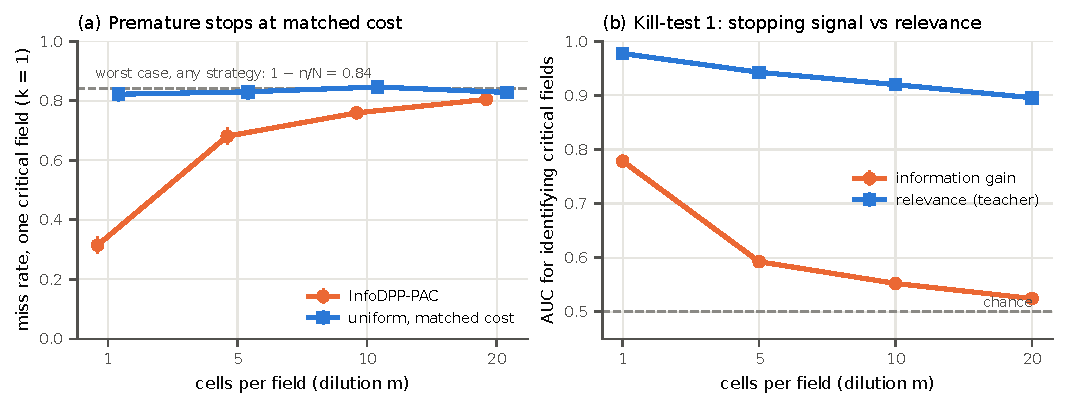
\includegraphics[width=\linewidth]{figures/fig1_partI.pdf}
\caption{Part I (RQ1), confirmatory run. (a) Miss rate with one critical field, for InfoDPP-PAC and for uniform sampling at the same per-episode cost (95\% Wilson intervals). Dashed: the worst-case bound $1-n/N$ for any strategy without location information (Theorem~\ref{thm:minimax}). (b) AUC of the information-gain term that drives stopping, and of the cell-level teacher's relevance score, for ranking critical above non-critical fields (95\% bootstrap intervals). The field-level teacher, trained on the pooled embeddings, reaches 0.978, 0.925, 0.882 and 0.827 at $m=1,5,10,20$ (text).}\label{fig:partI}
\end{figure}

\subsection{Certified threshold decisions (RQ3)}
The confirmatory run used 12,000 specimens, with 1,000 per value of $p$ for each threshold. Figure~\ref{fig:partIII} and Table~\ref{tab:hyp} summarise the results.
\begin{itemize}
\item \textbf{Validity (H3a).} All four valid designs passed at both thresholds. False certification at $p=\theta$ ranged from 0.001 to 0.022.
\item \textbf{Uncorrected adaptive selection (H3b).} The uncorrected design certified falsely in 0.993 (ICC, $\theta=0.10$) and 0.889 (WHO, $\theta=0.20$) of boundary specimens.
\item \textbf{Cost (H3c, H3d).} Classifier-driven betting needed fewer cells than ALPHA with uniform sampling at every $p>\theta$ (all Holm-adjusted $p<10^{-59}$). The median cells examined were:
  \begin{itemize}
  \item at $\theta=0.10$: 220 vs.\ 390 ($p=0.12$), 75 vs.\ 165 ($p=0.15$), 40 vs.\ 60 ($p=0.20$);
  \item at $\theta=0.20$: 335 vs.\ 445 ($p=0.22$), 145 vs.\ 250 ($p=0.25$), 60 vs.\ 105 ($p=0.30$).
  \end{itemize}
  Cost fell monotonically with the margin $|p-\theta|$. This comparison changes two things at once, the test and the sampler. Holding the test fixed, classifier-driven betting needed 0.28--0.73 times the cells of uniform betting (bootstrap intervals within $\pm0.03$). Holding the sampler fixed, the betting test needed 1.03--1.83 times the cells of ALPHA. In these 500-cell specimens, certification within 0.02 of the threshold required 44--89\% of the specimen; the next paragraph shows that this proportion is a consequence of the small population.
\item \textbf{Conventional counts.} A 100-cell count called ``above'' in 0.41 ($\theta=0.10$) and 0.43 ($\theta=0.20$) of specimens lying exactly on the threshold. It also called ``above'' in 0.14 and 0.24 of specimens 0.02 below the threshold.
\end{itemize}

\paragraph{Population size (exploratory).} Every cost above is capped at $M=500$. Repeating the designs at $M=1{,}000$, 2,000 and 4,000 cells (17,600 new specimens) left validity intact: false certification at $p=\theta$ was at most 0.040 at $\alpha=0.05$ and at most 0.007 at $\alpha=0.01$, for every design and $M$. Cost in cells, however, depends on the margin and hardly at all on $M$, once $M$ is large enough (Table~\ref{tab:mscale}). At a margin of 0.05 or more, the cells needed changed by at most 40\% between $M=1{,}000$ and 4,000, and at $M=4{,}000$ were within 20\% of Wald's large-population approximation $\log(1/\alpha)/\mathrm{KL}(p\,\|\,\theta)$ for a sequential probability ratio test with known alternative \cite{wald1945}. The approximation ignores both the gain from sampling without replacement and the cost of learning the alternative. Within 0.02 of the threshold, cost kept growing with $M$ towards that approximation (about 1,400 cells at $\theta=0.10$ and 2,500 at $\theta=0.20$). The fraction of the specimen examined fell as $M$ grew. ``Near-census'' is therefore a property of small specimens; the binding constraint is the number of cells, set by the margin. Classifier-driven sampling saved 36--65\% of the cells at every $M$, except at $p=0.22$ against $\theta=0.20$, where the saving was 19--23\% at $M\le1{,}000$ and vanished for $M\ge2{,}000$. Lowering $\alpha$ to 0.01 multiplied the cost of uniform ALPHA by 1.0--1.7. The 100-cell count called ``above'' in 40--45\% of boundary specimens at every $M$.

\begin{table}[t]
\centering\small
\caption{Median cells to certify $p>\theta$ against population size $M$ (exploratory; $\alpha=0.05$; 400 specimens per cell, $m=5$ cells per field). U: ALPHA with uniform sampling; C: betting with classifier-driven sampling. Approx.: $\log(1/\alpha)/\mathrm{KL}(p\|\theta)$. $^\dagger$Blast images reused, which affects only C.}\label{tab:mscale}
\begin{tabular}{@{}llrrrrrrrrr@{}}
\toprule
 & & \multicolumn{2}{c}{$M=500$} & \multicolumn{2}{c}{$M=1{,}000$} & \multicolumn{2}{c}{$M=2{,}000$} & \multicolumn{2}{c}{$M=4{,}000$} & \\
$\theta$ & $p$ & U & C & U & C & U & C & U & C & Approx.\\
\midrule
0.10 & 0.12 & 390 & 220 & 655 & 420 & 1,040 & 660 & 1,583 & 798 & 1,425\\
0.10 & 0.15 & 165 & 80 & 205 & 80 & 220 & 85 & 245$^\dagger$ & 85$^\dagger$ & 245\\
0.10 & 0.20 & 65 & 40 & 68 & 40 & 65 & 40 & 75$^\dagger$ & 40$^\dagger$ & 67\\
0.20 & 0.22 & 435 & 335 & 810 & 660 & 1,338 & 1,300 & 2,033$^\dagger$ & 2,043$^\dagger$ & 2,455\\
0.20 & 0.25 & 250 & 145 & 303 & 175 & 338$^\dagger$ & 190$^\dagger$ & 420$^\dagger$ & 185$^\dagger$ & 406\\
0.20 & 0.30 & 100 & 60 & 115 & 65 & 120$^\dagger$ & 65$^\dagger$ & 125$^\dagger$ & 70$^\dagger$ & 106\\
\bottomrule
\end{tabular}
\end{table}

\begin{figure}[t]
\centering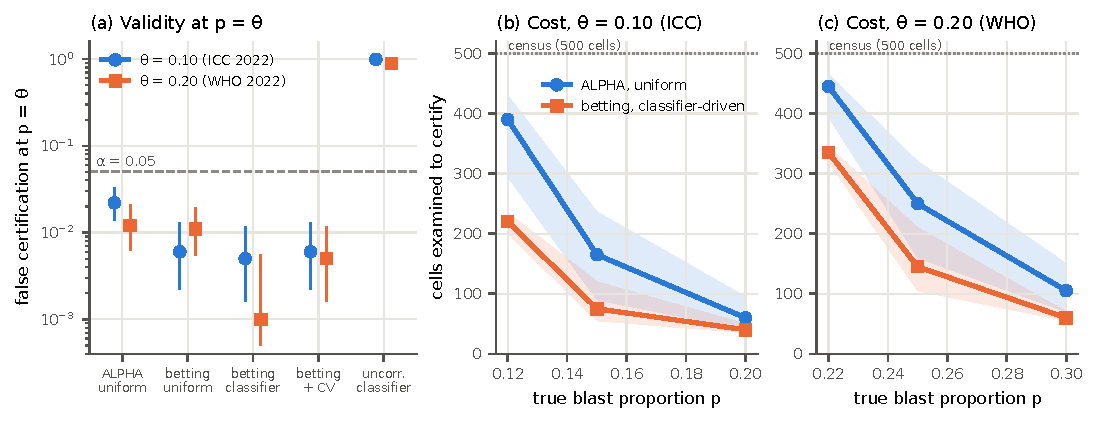
\includegraphics[width=\linewidth]{figures/fig3_partIII.pdf}
\caption{Part III (RQ3), confirmatory run (500-cell specimens; $\alpha=0.05$; designs paired on the same specimen). (a) False-certification rate at $p=\theta$ with 95\% Clopper--Pearson intervals, on a log scale. CV: control variate. The uncorrected design ranks fields by classifier score but analyses them as if uniformly sampled. (b, c) Median cells to certification, with interquartile bands; specimens that never certify are counted as 500 cells.}\label{fig:partIII}
\end{figure}

\subsection{Where the assumptions break (RQ4)}\label{sec:rq4}
\paragraph{Classifier error is not exchangeable (exploratory, KU-Optofil).}
\begin{itemize}
\item Blast recall at 95\% specificity varied across the 11 blast patients from 0.39 to 1.00 (homogeneity $\chi^2_{10}=61.1$, Monte-Carlo $p=0.0002$).
\item False-positive rates across blast-free patients were overdispersed 6.6-fold relative to a common binomial rate.
\item Errors concentrated in the immature granulocyte series and in lymphoid cells.
\item Within cell class, errors were associated with stain colour and contrast.
\end{itemize}
Certification remained valid even when blasts were drawn only from the low-recall patients (false certification $\le0.007$). Classifier-driven certification at $p=0.15$ then needed 2.3 times as many cells as with blasts from high-recall patients (140 vs.\ 60).

\paragraph{Acquisition shift (confirmatory, RV-PBS).} Applied unchanged to RV-PBS crops, the KU-trained probe's blast recall fell from 0.906 to 0.340 [0.250, 0.421] (H4a, supported), and its AUC from 0.979 to 0.786. Its false-positive rate did not rise: 0.058 [0.037, 0.081] vs.\ 0.050 (H4b, \textbf{not supported}). The certificate built on these shifted scores remained valid, with 3 false certifications in 1,000 specimens (H4c, supported). Efficiency, however, reversed. On fresh episodes (H6d, supported), classifier-driven sampling needed a median of 195 cells, against 110 for uniform sampling, at $p=0.20$ (paired Wilcoxon $p=1.5\times10^{-54}$). A plausible explanation is that a classifier which misses most blasts steers the sample away from them.

\paragraph{A defensive mixture (confirmatory).} We mixed classifier-driven sampling with 50\% uniform sampling ($q_t=\tfrac12 q^{\text{prop}}_t+\tfrac12 q^{\text{unif}}_t$). The test remained valid on both sources (false certification 0.001--0.014; H6a). In distribution, the mixture retained 58--73\% of the classifier-driven saving (H6c, supported). Under shift it reduced the excess cost at $p=0.20$ from $+77\%$ to $+23\%$ (ratio 1.23, 95\% CI [1.11, 1.30]). This missed the pre-registered bound of 1.20, so H6b was \textbf{not supported}. With a 25\% uniform share, the mixture gave essentially no protection under shift (ratio 1.73).

\paragraph{Spatial clustering and the unit of analysis.} We placed blasts in a few ``hot'' fields of 5 cells, at nominal densities of 0.6 and 1.0, so that clustering was strong (E3.1, confirmatory, 18,000 specimens).
\begin{itemize}
\item The three field-level designs remained valid in all 36 pre-registered cells, with a maximum false-certification rate of 0.042 (H5a).
\item Analysing the cells of uniformly sampled fields \emph{as if each had been drawn individually} was valid when blasts were scattered (0.029 and 0.041). It certified falsely in 0.327 [0.298, 0.357] ($\theta=0.10$) and 0.478 [0.447, 0.509] ($\theta=0.20$) of boundary specimens under the strongest clustering (H5b).
\item Clustering doubled the cost of uniform field sampling, from 160 to 345 cells at $p=0.15$, $\theta=0.10$ (H5c). It lowered the cost of classifier-driven sampling, from 80 to 55 cells, because the classifier finds the hot fields.
\end{itemize}

\paragraph{Clustering in real smears (confirmatory, BoneMarrowWSI).} The eligible data comprised 75 patients, 116 fully labelled regions of interest, 9,375 nucleated cells and 5,841 blasts.
\begin{itemize}
\item Blasts were clustered within regions (H7a, supported). The intraclass correlation across the four quadrants of a region (about $113\,\mu$m) was 0.032 [0.016, 0.050] (permutation $p=0.024$). At the $4\times4$ scale (about $56\,\mu$m) it was 0.098 (permutation $p=0.0005$). Nearest-neighbour blast enrichment was also significant ($p=0.0005$).
\item No difference between the two regions of a patient was detected.
\item After the run we noticed that the permutation null of the ANOVA estimator is not centred at zero: its mean is 0.018 at the quadrant scale. The excess clustering (about 0.014) is therefore smaller than the raw estimate. The permutation test is unaffected. We report this as an exploratory correction.
\item In a pre-specified Beta-binomial model with 17 cells per field, the measured clustering implies that the cell-level mis-analysis certifies falsely in 0.043--0.070 ($\theta=0.10$) and 0.051--0.103 ($\theta=0.20$) of boundary specimens across the ICC's confidence range. Field-level analysis stayed $\le0.014$.
\item On the same ICC scale, the E3.1 stress arrangements (0.5--1.0) are one to two orders of magnitude more clustered than these monolayer regions (Figure~\ref{fig:rq4}b).
\end{itemize}

\paragraph{Unequal field sizes (exploratory).} Real fields differ in size: BoneMarrowWSI quadrants hold 12--29 nucleated cells (interquartile range; coefficient of variation 0.62). In real regions, the mean of quadrant proportions differed from the region's blast proportion by $-0.004$ on average $[-0.008,0.001]$ (patient bootstrap, 116 regions). Proportion and size were barely related (within-region Spearman correlation 0.04), but the difference exceeded 0.03 in absolute value in 10\% of regions. In simulated specimens with these field sizes (about 1,300 cells), averaging field proportions with ALPHA certified falsely in 0.38 $[0.35,0.41]$ ($\theta=0.10$) and 0.32 $[0.29,0.35]$ ($\theta=0.20$) of boundary specimens, even with blasts placed independently of size. With blasts enriched in small fields it certified falsely in every specimen. The reason is that the analysis tests the mean of proportions, which exceeds $\theta$ in about half of the specimens with $p=\theta$; the test is valid for that quantity, but it is the wrong quantity. Both constructions of Proposition~\ref{prop:unequal} stayed valid in every condition, with false certification at most 0.005. They differ in cost. With known counts, classifier-driven sampling certified $p=0.15$ against $\theta=0.10$ with a median of 297 cells (23\% of the specimen), and uniform sampling with 646. The bounded assorter with $m_{\max}=91$, the largest quadrant observed, needed 631 cells with betting and 1,031 with ALPHA, because the bound shrinks the margin by $\bar m/m_{\max}\approx0.24$. Recording each field's cell count, which needs a detector but not a classifier, is therefore worth a large saving.

\begin{figure}[t]
\centering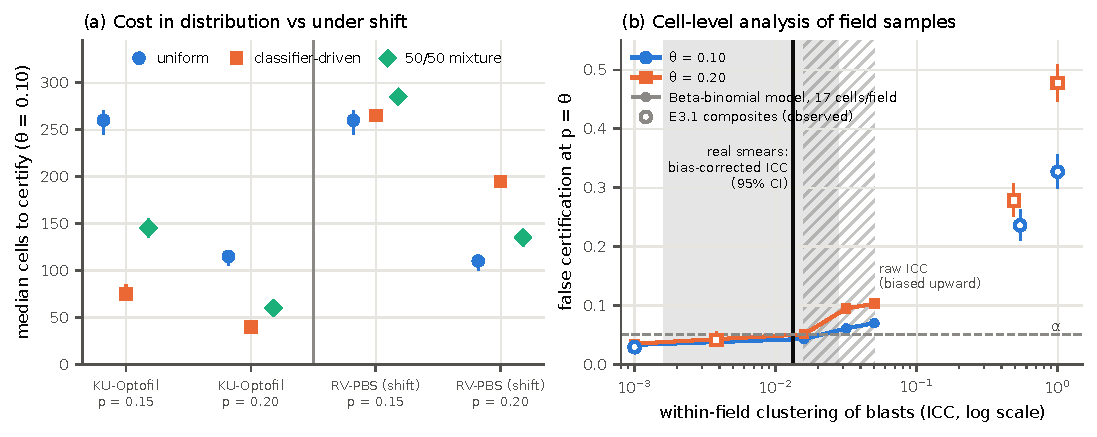
\includegraphics[width=\linewidth]{figures/fig4_rq4.pdf}
\caption{RQ4. (a) Median cells to certify $p>0.10$ in distribution (KU-Optofil, cross-fitted scores) and under acquisition shift (RV-PBS, KU-trained probe); 95\% bootstrap intervals. All designs keep false certification $\le0.014$. (b) False certification at $p=\theta$ when the cells of sampled fields are analysed as individual draws. Open markers: composites with scattered or hot-field arrangements (5 cells per field). Lines: model at the clustering measured in real bone-marrow regions (17 cells per field). Grey band: 95\% CI of the raw ICC, which is biased upward. ICC values of 0 are plotted at $10^{-3}$.}\label{fig:rq4}
\end{figure}

\begin{table}[t]
\centering\small
\caption{Pre-registered hypotheses and verdicts. All confirmatory data were generated after the corresponding protocol was frozen (Appendix~\ref{app:audit}). Type: E, an empirical claim; V, a check of the implementation or of a property that holds by theorem.}\label{tab:hyp}
\begin{tabular}{@{}lllp{7.6cm}l@{}}
\toprule
RQ & ID & Type & Hypothesis (abridged) & Verdict\\
\midrule
1 & H1a & V & InfoDPP-PAC stop point independent of rarity & supported\\
1 & H1b & E & Advantage over matched-cost uniform shrinks with dilution & supported (4/4)\\
1 & H1c & E & No advantage ($\pm0.05$) at $m\ge10$, $k=1$ & \textbf{not supported}\\
2 & H1d & V & Uniform miss rate equals $1-n/N$ & supported\\
1 & KT1 & E & Information gain and relevance are separable signals & supported\\
3 & H3a & V & All four designs valid at both thresholds & supported\\
3 & H3b & E & Uncorrected adaptive selection invalid & supported\\
3 & H3c & E & Classifier-driven sampling cheaper than uniform & supported\\
3 & H3d & E & Cost decreases with the margin & supported\\
4 & H4a & E & Blast recall drops under acquisition shift & supported\\
4 & H4b & E & False-positive rate rises under shift & \textbf{not supported}\\
4 & H4c & V & Certificate valid with shifted side information & supported\\
4 & H5a & V & Field-level tests valid under clustering & supported\\
4 & H5b & E & Cell-level analysis of field samples invalid under clustering & supported\\
4 & H5c & E & Clustering raises the cost of valid certification & supported\\
4 & H6a & V & Defensive mixture valid & supported\\
4 & H6b & E & Mixture caps loss under shift below 20\% & \textbf{not supported}\\
4 & H6c & E & Mixture keeps $\ge50\%$ of in-distribution saving & supported\\
4 & H6d & E & Cost reversal under shift replicates & supported\\
4 & H7a & E & Blasts spatially clustered in real smears & supported\\
\bottomrule
\end{tabular}
\end{table}

\section{Discussion}
\paragraph{What is guaranteed, and by what.} Our results separate three quantities that are often reported together:
\begin{itemize}
\item \emph{Model confidence} about examined fields, which says nothing about unexamined ones.
\item \emph{Information saturation}, which concerns the selector's representation of the specimen, not the decision-relevant evidence. Its association with that evidence can disappear, as it did here once cells were pooled into fields, even though the pooled representation still carried the evidence.
\item \emph{Design-based certification}, which bounds the probability of a false threshold decision for the specific specimen, provided the selection probabilities are known and positive and the labels come from verification.
\end{itemize}
Only the third is a guarantee about what was not examined, and it held in every condition we tested, including a classifier that lost two thirds of its blast recall. Classifier quality determined only how quickly certification was reached, and could make it slower than uniform sampling.

\paragraph{Practical implications.}
\begin{itemize}
\item Certify a proportion against a stated threshold rather than the presence or absence of rare cells; the latter requires a near-census (Theorem~\ref{thm:minimax}). The cost of the former is set by the margin to the threshold, in cells, not by the size of the specimen: at a margin of 0.05, 165--420 cells with uniform sampling and 80--190 with classifier-driven sampling. Within 0.02 of the threshold it exceeded 1,000 cells whenever the specimen held 2,000 or more.
\item Record selection probabilities, and never analyse adaptively selected fields as if they had been sampled uniformly.
\item Analyse at the unit that was sampled. Treating the cells of a sampled field as independent draws is anti-conservative whenever blasts cluster. The effect is modest in the evenly dispersed monolayer we measured and severe under strong clustering. When fields differ in size, do not average field proportions: weight fields by their cell counts if they are known, or use the bounded assorter of Proposition~\ref{prop:unequal}.
\item Mixing a fixed uniform share into classifier-driven sampling limits, but does not remove, the efficiency loss under shift.
\end{itemize}

\paragraph{Limitations.}
\begin{itemize}
\item Most specimens are composites of single-cell images from one laboratory. A composite specimen mixes cells from several patients, so it is not a real patient's smear, and all blasts in Parts I and III come from 11 patients. Results varied across patient folds, and intervals over five folds or 11 patients are themselves imprecise. How large InfoDPP-PAC's residual advantage is depends on how the background is composed (pooled or single-host).
\item The external blood dataset is small, lacks patient identifiers, and was cropped by our own rule, which confounds stain and camera effects with framing.
\item The real-smear spatial analysis uses pediatric bone-marrow aspirates, not peripheral blood. Its regions were chosen in the evenly dispersed monolayer, so clustering elsewhere in a smear may be larger. The consequence for validity at the measured clustering comes from a model, not from observed certification rates.
\item Verification is simulated with expert labels ($\beta=0$).
\item The population-size, unequal-field and field-level-teacher analyses were added after the pre-registered analyses and are exploratory.
\item InfoDPP-PAC's unreported hyperparameters were calibrated to its reported cost, so our reimplementation may differ from the authors' configuration.
\item We used a single frozen encoder.
\item We did not implement prediction-powered e-values \cite{csillag2025ppe}.
\end{itemize}

\section{Conclusion}
When an adaptive system decides how much of a blood smear to examine, information saturation does not certify what remains unexamined. Without location information, certifying the absence of rare evidence requires examining nearly all of the specimen, whatever the strategy. Threshold decisions about the blast proportion, by contrast, can be certified with finite-sample, anytime-valid guarantees whose validity rests on the sampling design and the unit of analysis rather than on the classifier. Extending this analysis to fully annotated peripheral-blood smears, and to verification by haematologists, is the most important next step.

\paragraph{Data and code availability.} All code, the pre-registration and its git history, the audit trail of Appendix~\ref{app:audit} and the analysis outputs are available at [repository URL; to be archived on Zenodo with a DOI at submission]. KU-Optofil and BoneMarrowWSI-PediatricLeukemia are public datasets under CC BY 4.0. RV-PBS is publicly distributed by its authors without a stated licence and was used for research only.

\paragraph{Acknowledgements.} The author thanks Dr.\ Bal\'azs Harangi for supervising this work. [Further acknowledgements to be added.]

\bibliographystyle{unsrtnat}
\bibliography{refs}

\appendix
\section{Proof of Theorem~\ref{thm:minimax}}\label{app:proof}
Fix $x$ and a realisation $u$ of the examiner's independent randomness $U$.

\emph{Step 1 (the all-negative path).} Consider the run in which every examined field is negative. Every input to the policy is then determined by $(x,u)$, so the run examines a fixed sequence $a_1(u),\dots,a_{n'}(u)$ with $n'\le n$. Let $A(u)$ be the set of these fields.

\emph{Step 2 (the miss event is determined by $A(u)$).} If $C\cap A(u)=\emptyset$, every field on the all-negative path is negative under $C$, so the actual run follows that path and misses $C$. Otherwise, let $t$ be the first index with $a_t(u)\in C$. Up to step $t-1$ all observations are negative, so the actual run follows the all-negative path through step $t$, examines $a_t(u)\in C$, and does not miss. Hence $\Prb_\pi(M_n\mid x,C)=\Prb_U(C\cap A(U)=\emptyset)$.

\emph{Step 3 (averaging over placements).} Let $C$ be uniform over the $k$-subsets, independent of $U$; Assumption~\ref{ass:A} makes every such $C$ admissible. For fixed $u$, the fraction of $k$-subsets disjoint from $A(u)$ is $\binom{N-|A(u)|}{k}/\binom{N}{k}\ge\binom{N-n}{k}/\binom{N}{k}=h(N,k,n)$, using $\binom{N-n}{k}/\binom{N}{k}=\binom{N-k}{n}/\binom{N}{n}$. Averaging over $U$ gives $\E_C\Prb_\pi(M_n\mid x,C)\ge h(N,k,n)$.

\emph{Step 4 (worst case is at least the average).} $\max_C\Prb_\pi(M_n\mid x,C)\ge\E_C\Prb_\pi(M_n\mid x,C)\ge h(N,k,n)$. Uniform sampling achieves $h$ for every $C$ by Proposition~\ref{prop:uniform}.

For a deterministic policy, $A$ is a single set with $|A|\le n\le N-k$. Placing $C$ inside $[N]\setminus A$ gives miss probability 1. \qed

\section{Deviations from the protocol and from the reimplemented method}\label{app:dev}
\begin{itemize}
\item \textbf{InfoDPP-PAC.} We used DINOv2 ViT-S/14 instead of the paper's Phikon (H\&E) encoder, because there is no established open Wright--Giemsa encoder. $\tau$ was calibrated to the reported operating point, and $\rho=1$. A field is the mean of its cells' embeddings. The ``fixed-order'' baseline is not a spatial raster.
\item \textbf{Part III.} An early exploratory construction fed importance-weighted draws into ALPHA's unweighted null-mean update, which is not a valid supermartingale. It was withdrawn before the confirmatory protocol and replaced by the construction of Shekhar et al.\ \cite{shekhar2023rlfa}.
\item \textbf{Part I analysis.} An exploratory batch-overwrite bug, found before the protocol was frozen, had caused early estimates to use three of five folds. It was corrected.
\item \textbf{Real-smear spatial analysis.} The analyses were run with byte-identical frozen scripts, in a different compute environment because of time limits (SHA-256 hashes recorded). The bias of the ICC estimator was noticed after the run and is reported as exploratory.
\item \textbf{Teacher.} InfoDPP-PAC's teacher $T(x_i)$ acts on the patch embedding. Our pre-registered runs used the largest cross-fitted cell-level score in a field, which presupposes cell detection. A field-level teacher trained on pooled embeddings was added afterwards (exploratory); it changed InfoDPP-PAC's miss rates by at most 0.04 and lowered the relevance AUC at $m=20$ from 0.896 to 0.827.
\item \textbf{Sensitivity analyses.} The four pre-registered sensitivity analyses (seeds 20260402--20260405) were run after the main analyses, on 2026-10-19, with the frozen script. An earlier draft had instead cited exploratory runs that reused the main run's random streams. The $\tau$ sweep was run at $k=1$ only, because the protocol does not state its grid. The pre-registered patient-level bootstrap could not be computed from the frozen outputs, which do not record the source patient of each blast; fold-level intervals are reported instead, and the field-level-teacher episodes record patients.
\item \textbf{Episode counts.} An earlier draft reported 15,000 E3.1 and 5,000 E3.2 specimens. The output files contain 18,000 and 4,500, as Amendment 3 specifies; only the reported totals change.
\item \textbf{Typed dates.} Several freeze dates typed in the protocol text are wrong (for example 2026-09-26 for tags created on 2026-09-25). They are left unedited so that the text matches the tags; Appendix~\ref{app:audit} gives the times from git.
\item \textbf{Not implemented.} Prediction-powered e-values; haematologist verification.
\end{itemize}

\section{Pre-registration audit trail}\label{app:audit}
Times are UTC. Push times are from the local record of pushes to the remote repository, which the hosting service records independently. Output times are file modification times, because result files are not under version control; they are weaker evidence. The frozen scripts and \texttt{src/} are unchanged since their tags.

\begin{center}\small
\begin{tabular}{@{}llllr@{}}
\toprule
Tag & Commit & Pushed & First confirmatory output & Gap\\
\midrule
\texttt{prereg-v1} & b3f114d & 2026-09-25 10:14:53 & none (amended before any run) & --\\
\texttt{prereg-v1.1} & db4463d & 2026-09-25 10:51:18 & Part I, 10:52:01 & 43\,s\\
\texttt{prereg-v2} & fc4f1e8 & 2026-09-25 11:36:43 & Part III, 11:55:08; RV-PBS, 11:59:27 & 18\,min\\
\texttt{prereg-v3} & f014352 & 2026-09-25 12:39:59 & E3.1, 12:41:27 & 1.5\,min\\
\texttt{prereg-v4} & 40c838d & 2026-09-30 10:22:17 & BoneMarrowWSI, 10:26:58 & 4.7\,min\\
\bottomrule
\end{tabular}
\end{center}
Content hashes of all confirmatory outputs are listed in \texttt{docs/PREREG\_AUDIT.md}. Re-running one Part I cell in a separate environment reproduced the stored episodes: miss indicators were identical, and two of 1,000 stop steps differed by one field because $\tau$ differed in the sixth significant digit.

\end{document}
